%% Vision Agent Architecture Report
%% DisasterAI — Advanced Deep Learning · Esprit 5DS1 · 2026-27
%% Compile: pdflatex vision_agent_report.tex

\documentclass[11pt, a4paper]{article}

%% ─── Packages ────────────────────────────────────────────────────────────────
\usepackage[top=2.3cm, bottom=2.3cm, left=2.4cm, right=2.4cm]{geometry}
\usepackage[T1]{fontenc}
\usepackage{times}
\usepackage{microtype}
\usepackage{xcolor}
\usepackage{booktabs}
\usepackage{array}
\usepackage{enumitem}
\usepackage{caption}
\usepackage{amsmath}
\usepackage{tikz}
\usetikzlibrary{shapes.geometric, arrows.meta, positioning, calc}
\usepackage[hidelinks]{hyperref}
\usepackage{titlesec}
\usepackage{fancyhdr}
\usepackage{graphicx}

%% ─── Grayscale-only palette (no colour anywhere in the document) ────────────
\definecolor{dgray}{gray}{0.35}
\definecolor{mgray}{gray}{0.55}
\definecolor{lgray}{gray}{0.85}
\definecolor{vlgray}{gray}{0.94}

%% ─── Section numbering, headers ──────────────────────────────────────────────
\titleformat{\section}{\normalfont\large\bfseries}{\thesection}{0.6em}{}
\titleformat{\subsection}{\normalfont\bfseries}{\thesubsection}{0.6em}{}
\pagestyle{fancy}
\fancyhf{}
\renewcommand{\headrulewidth}{0.4pt}
\fancyhead[L]{\small\textsc{Vision Agent Architecture Report}}
\fancyhead[R]{\small DisasterAI}
\fancyfoot[C]{\small\thepage}

\setlength{\parskip}{3pt}
\newcommand{\code}[1]{\texttt{\small#1}}

%% ─── TikZ node styles (grayscale, shade-coded instead of colour-coded) ──────
\tikzset{
  box/.style={rectangle, rounded corners=2pt, draw=black, thick,
              minimum width=3.4cm, minimum height=0.9cm, align=center, font=\small},
  wide/.style={rectangle, rounded corners=2pt, draw=black, thick,
               minimum width=7.4cm, minimum height=0.9cm, align=center, font=\small},
  primary/.style={fill=white},
  secondary/.style={fill=lgray},
  tertiary/.style={fill=vlgray},
  arr/.style={-Stealth, thick, draw=black},
  darr/.style={-Stealth, thick, dashed, draw=dgray},
}

\begin{document}
\pagenumbering{arabic}

%% ─── Title ───────────────────────────────────────────────────────────────────
\begin{center}
  {\LARGE\bfseries Vision Agent: A Dual-Encoder Architecture for\\[2pt]
   Disaster Image Classification}\\[10pt]
  {\large DisasterAI --- Multi-Agent Disaster Assessment System}\\[4pt]
  {\normalsize Advanced Deep Learning \quad\textbar\quad Esprit 5DS1 \quad\textbar\quad 2026--27}
\end{center}

\vspace{6pt}
\begin{center}
\begin{minipage}{0.88\textwidth}
\small\noindent\textbf{Abstract.} We present the Vision Agent, the perceptual module of a
multi-agent disaster-assessment pipeline. Given a single image, the system produces a
five-way classification (\emph{fire}, \emph{flood}, \emph{normal}, \emph{irrelevant},
\emph{uncertain}), a natural-language description, and an explicit reliability estimate.
Classification is performed by a cloud-hosted vision-language model (Qwen, served through
Groq, with a local fallback), queried independently on three test-time-augmented views of
the input image. Agreement across the three views yields a stability score that is combined
with a self-supervised visual-similarity signal from a frozen DINOv2 encoder to produce a
final reliability verdict. We describe the architecture, the rationale behind each design
choice, and report results from controlled runs on held-out images from the project's fire,
flood, and normal classes, each achieving unanimous three-way agreement and a reliable
verdict.
\end{minipage}
\end{center}

\vspace{4pt}

%% ─── 1. Introduction ─────────────────────────────────────────────────────────
\section{Introduction}

The Vision Agent is one of five cooperating agents in the DisasterAI pipeline (Incident,
Vision, Knowledge/RAG, Risk, Report). Its task is narrow but safety-critical: given an image
submitted alongside an incident report, decide whether it shows an active fire, an active
flood, an unaffected (``normal'') scene, content unrelated to disaster assessment
(\emph{irrelevant}), or content too ambiguous to classify (\emph{uncertain}), and attach a
reliability estimate that downstream agents can condition on. A wrong but confident answer is
more harmful to the pipeline than a correct abstention, which motivated most of the design
decisions described below.

%% ─── 2. System Architecture ──────────────────────────────────────────────────
\section{System Architecture}
\label{sec:architecture}

Figure~\ref{fig:arch} shows the full pipeline. Two branches run on the same input image: a
\emph{semantic} branch (test-time augmentation followed by a vision-language model) and a
\emph{visual-similarity} branch (a frozen DINOv2 encoder). Their outputs are combined by a
Visual Consistency Module and a Reliability Layer before the agent returns a single,
schema-validated result.

\begin{figure}[h]
\centering
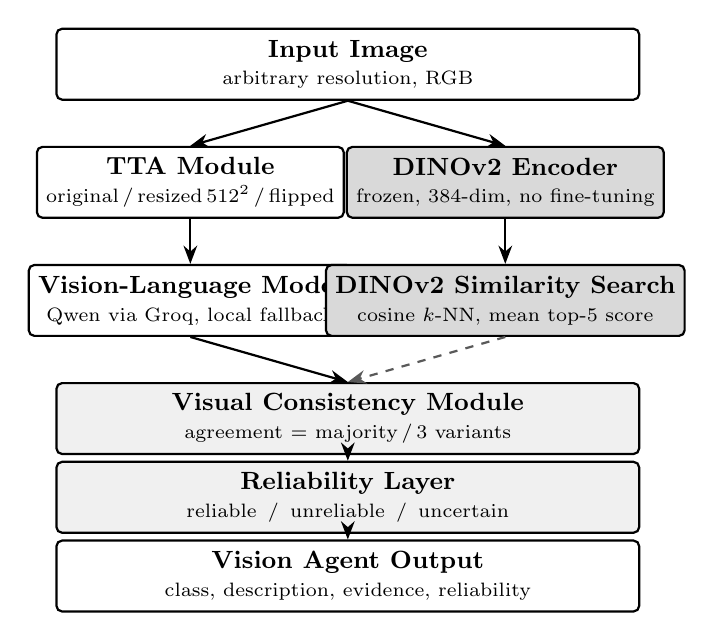
\begin{tikzpicture}[
    every node/.style={font=\small},
    yscale=1, xscale=1
  ]

  %% ---- Row 0: input (centered column, x = 0) ----
  \node[wide, primary] (input) at (0, 0)
    {\textbf{Input Image}\\[-1pt]{\scriptsize arbitrary resolution, RGB}};

  %% ---- Row 1: the two branches, symmetric about x = 0 ----
  \node[box, primary]   (tta)  at (-2.0, -1.5)
    {\textbf{TTA Module}\\[-1pt]{\scriptsize original\,/\,resized\,512\textsuperscript{2}\,/\,flipped}};
  \node[box, secondary] (dino) at ( 2.0, -1.5)
    {\textbf{DINOv2 Encoder}\\[-1pt]{\scriptsize frozen, 384-dim, no fine-tuning}};

  %% ---- Row 2: the two branches continue ----
  \node[box, primary]   (vlm) at (-2.0, -3.0)
    {\textbf{Vision-Language Model}\\[-1pt]{\scriptsize Qwen via Groq, local fallback}};
  \node[box, secondary] (sim) at ( 2.0, -3.0)
    {\textbf{DINOv2 Similarity Search}\\[-1pt]{\scriptsize cosine $k$-NN, mean top-5 score}};

  %% ---- Rows 3--5: merge back onto the centered column ----
  \node[box, tertiary, minimum width=7.4cm] (consist) at (0, -4.5)
    {\textbf{Visual Consistency Module}\\[-1pt]{\scriptsize agreement $=$ majority\,/\,3 variants}};
  \node[box, tertiary, minimum width=7.4cm] (rel) at (0, -5.5)
    {\textbf{Reliability Layer}\\[-1pt]{\scriptsize reliable \,/\, unreliable \,/\, uncertain}};
  \node[wide, primary] (out) at (0, -6.5)
    {\textbf{Vision Agent Output}\\[-1pt]{\scriptsize class, description, evidence, reliability}};

  %% ---- Arrows ----
  \draw[arr] (input.south) -- (tta.north);
  \draw[arr] (input.south) -- (dino.north);
  \draw[arr] (tta.south) -- (vlm.north);
  \draw[arr] (dino.south) -- (sim.north);
  \draw[arr]  (vlm.south) -- (consist.north);
  \draw[darr] (sim.south) -- (consist.north);
  \draw[arr] (consist.south) -- (rel.north);
  \draw[arr] (rel.south) -- (out.north);

\end{tikzpicture}
\caption{Vision Agent pipeline. White nodes: the semantic (language) branch. Gray nodes: the
non-linguistic visual-similarity branch. The dashed arrow denotes a shadow-mode signal: it is
logged alongside the reliability verdict but, in the default configuration, does not alter it.}
\label{fig:arch}
\end{figure}

%% ─── 3. Components ───────────────────────────────────────────────────────────
\section{Component Design}

\subsection{Vision-Language Model: Cloud-First with Local Fallback}

The semantic branch is served by a hosted multimodal model (\emph{Qwen}, accessed through the
Groq inference API) with a local model (served through Ollama) configured as an offline
fallback. Model selection is a single configuration value; no code change is required to
switch providers.

\paragraph{Rationale.} Three considerations drove this choice over a purely local deployment.
First, output quality: in side-by-side comparisons on the project's test images, the
cloud-hosted model produced substantially more specific and better-grounded descriptions than
the local alternative (Table~\ref{tab:quality}). Second, deployment cost: a cloud API requires
no GPU, no model download, and no local inference service, which matters directly for handing
the system to a collaborator's machine, where disk space and GPU availability cannot be
assumed. Third, resilience: request failures are retried automatically, including honoring the
provider's rate-limit back-off interval, before falling back to the secondary provider.

\begin{table}[h]
\centering\small
\begin{tabular}{p{2.6cm}p{5.0cm}p{5.0cm}}
\toprule
& \textbf{Local (Ollama)} & \textbf{Cloud (Qwen via Groq)} \\
\midrule
Description  & ``A wildfire is burning in the mountains.'' &
``Intense orange flames burn along a ridge line, generating a massive plume of thick, dark
smoke.'' \\
Evidence     & generic (flames, smoke, structural collapse) &
specific (active flames along a ridge, thick dark smoke plume, glowing embers and fire front)\\
Deployment   & requires local GPU, model download & requires only an API key \\
\bottomrule
\end{tabular}
\caption{Output quality and deployment cost, same input image, two VLM backends.}
\label{tab:quality}
\end{table}

\paragraph{Query design.} Each call asks for a single structured JSON object containing the
predicted class, a natural-language description, and a short evidence list, in one pass. An
earlier iteration issued three separate questions (classification, evidence, description) and
occasionally produced internally inconsistent answers --- a classification of \emph{fire}
accompanying a description of a lake. Merging the three sub-answers into one constrained JSON
response removes this failure mode by construction: class and description are now necessarily
drawn from the same reasoning pass.

\subsection{Five-Way Classification Taxonomy}
\label{sec:taxonomy}

The agent distinguishes five outcomes, listed in Table~\ref{tab:taxonomy}. The
\emph{normal}/\emph{irrelevant} distinction is deliberate: a street, building, or landscape
with no active incident is still within the domain the pipeline is meant to assess
(\emph{normal}), whereas a selfie, a document photograph, or an unrelated object is not
(\emph{irrelevant}). Separating the two allows the pipeline to reject out-of-domain input
early rather than force it into a disaster-relevant answer.

\begin{table}[h]
\centering\small
\begin{tabular}{p{2.0cm}p{9.6cm}}
\toprule
\textbf{Class} & \textbf{Definition} \\
\midrule
fire       & active flames, burning structures or vegetation, wildfire smoke columns \\
flood      & water inundation --- flooded streets, submerged vehicles or buildings, overflowing rivers \\
normal     & a disaster-relevant scene (street, building, landscape, vehicle, person) with no active incident \\
irrelevant & content unrelated to disaster assessment entirely --- a selfie, a document, a screenshot, an unrelated object \\
uncertain  & the image is too dark, blurred, or ambiguous to classify with confidence \\
\bottomrule
\end{tabular}
\caption{Classification taxonomy. The boundary between \emph{normal} and \emph{irrelevant} is
established purely through the natural-language class definitions given to the model; no
separate rule-based gate exists ahead of the language model call.}
\label{tab:taxonomy}
\end{table}

\subsection{Test-Time Augmentation}

Each image is independently classified in three forms: the original, a version resized to
$512\times512$, and a horizontally mirrored version. Running the same query three times on
perturbed inputs exposes a form of prediction instability that a single call cannot reveal. The
three transformations were chosen so as not to destroy the physical evidence being searched
for: a vertical flip would place smoke below ground and water above it; a rotation would change
the frame of reference the model is implicitly conditioned on; a colour transform could remove
fire's characteristic spectral signature. None of the three is applied.

\subsection{DINOv2 Visual Similarity}

The second branch extracts a 384-dimensional embedding from a frozen DINOv2 vision transformer
(no fine-tuning, no gradient computation) and compares it, by cosine similarity, against a
small reference set of previously encoded images. The resulting mean top-5 similarity is a
purely visual signal: it contains no natural language and cannot be subject to the same class
of hallucination that affects the vision-language model. It is reported as part of the
reliability block but, in the default (\emph{shadow}) mode, never changes the predicted class
or the reliability verdict on its own; the system is configured to require a corroborating
signal (low test-time-augmentation agreement) before the similarity score is allowed to
downgrade a result.

\subsection{Visual Consistency Module and Reliability Layer}

The three test-time-augmentation answers are reduced to an agreement score, the fraction of
variants agreeing with the majority class ($1/3$, $2/3$, or $3/3$). An agreement score below
a fixed threshold ($2/3$), or the presence of hedging language in the model's own answer, marks
the result \emph{unreliable}; in that case, the final predicted class is deliberately replaced
with \emph{uncertain} rather than reported as the (unstable) majority vote. This design decision
reflects the project's governing principle: a confident wrong answer is more dangerous, in a
disaster-assessment context, than an honest abstention.

%% ─── 4. Experimental Results ─────────────────────────────────────────────────
\section{Experimental Results}
\label{sec:results}

Three images, one from each of the project's labelled classes (\emph{fire}, \emph{flood},
\emph{normal}), were drawn from the training corpus and passed through the complete pipeline
with the cloud vision-language model active. Table~\ref{tab:results} summarises the outcome of
each run; all three produced unanimous agreement across the three test-time-augmented variants
and were marked reliable.

\begin{table}[h]
\centering\small
\begin{tabular}{llccc}
\toprule
\textbf{Image} & \textbf{Predicted class} & \textbf{TTA agreement} & \textbf{Reliability} & \textbf{DINOv2 mean sim.} \\
\midrule
\code{fire\_image0001.jpg}  & fire   & 3/3 (1.00) & reliable & 0.859 \\
\code{flood\_image0001.jpg} & flood  & 3/3 (1.00) & reliable & 0.784 \\
\code{image\_5990.png}      & normal & 3/3 (1.00) & reliable & 0.887 \\
\bottomrule
\end{tabular}
\caption{Results of three controlled runs, one per class, using the cloud vision-language model
(Qwen via Groq). TTA agreement is reported as (agreeing variants)/(total variants).}
\label{tab:results}
\end{table}

\paragraph{Fire.} All three variants converged on the same evidence set: ``active flames along
a ridge,'' ``thick dark smoke plume,'' ``glowing embers and fire front.'' The canonical
description reads: \emph{``Intense orange flames burn along a ridge line, generating a massive
plume of thick, dark smoke.''} The five nearest neighbours retrieved by the DINOv2 similarity
search were themselves all fire images, corroborating the classification through an entirely
independent, non-linguistic signal.

\paragraph{Flood.} The model consistently identified ``muddy brown water covering the ground,''
submerged trees with only their canopies visible, and buildings with only their roofs above the
waterline, across all three augmented variants, with only minor paraphrasing between runs. Mean
DINOv2 similarity (0.784) was lower than for the fire example, consistent with flood scenes
exhibiting more visual heterogeneity (aerial versus street-level framing, vegetation density,
water turbidity) than the comparatively uniform visual signature of active flame and smoke.

\paragraph{Normal.} A photograph of a high-rise building against a sunset sky was correctly
classified as \emph{normal} in all three variants, with an empty evidence list in each case ---
the expected behaviour for this class under the prompt design of Section~\ref{sec:taxonomy},
since \emph{normal} and \emph{irrelevant} are defined to carry no fire/flood evidence items.
Mean DINOv2 similarity (0.887) was the highest of the three runs; its nearest neighbours were
exclusively other \emph{normal}-labelled images.

\paragraph{Scope of this evaluation.} These three runs demonstrate correct, stable, and
reliable behaviour on held-out examples of each labelled class under the current cloud
vision-language backend. They do not constitute a full accuracy benchmark: a quantitative
evaluation across a larger, randomly sampled test set, and an explicit test of the
\emph{irrelevant} and \emph{uncertain} classes on genuinely out-of-domain images (which the
present dataset does not contain), remain open work.

%% ─── 5. Discussion and Limitations ───────────────────────────────────────────
\section{Discussion and Limitations}

Two limitations are worth stating plainly. First, the \emph{normal}/\emph{irrelevant} boundary
(Section~\ref{sec:taxonomy}) has not yet been exercised on a genuinely out-of-domain image ---
every test to date has used fire, flood, or normal-disaster-scene photographs from the project
corpus, none of which approximate a selfie or a document photograph. Second, the DINOv2
reference store used in these experiments is small (built from a limited subset of the
project's images); the reported similarity scores are internally consistent but should not be
read as calibrated probabilities. Both points are natural next steps rather than defects in the
present design.

%% ─── References ──────────────────────────────────────────────────────────────
\vspace{4pt}
\begin{thebibliography}{9}
\small

\bibitem{bai2023qwenvl}
  J.\ Bai et al.
  \textit{Qwen-VL: A Versatile Vision-Language Model for Understanding, Localization, Text
  Reading, and Beyond}.
  arXiv:2308.12966, 2023.

\bibitem{shanmugam2021tta}
  D.\ Shanmugam et al.
  \textit{Better Aggregation in Test-Time Augmentation}.
  ICCV 2021.

\bibitem{brown2020fewshot}
  T.\ Brown et al.
  \textit{Language Models are Few-Shot Learners}.
  NeurIPS 2020.

\bibitem{oquab2023dinov2}
  M.\ Oquab et al.
  \textit{DINOv2: Learning Robust Visual Features without Supervision}.
  TMLR 2024.

\bibitem{wei2022cot}
  J.\ Wei et al.
  \textit{Chain-of-Thought Prompting Elicits Reasoning in Large Language Models}.
  NeurIPS 2022.

\end{thebibliography}

\end{document}
